\documentclass{standalone}
% Shared figure style: the paper's typefaces, sizes and the two-colour encoding.
% Identical copies live in every figure directory so that each builds on its own.
\usepackage{fontspec}
\setmainfont{LinLibertine}[Extension=.otf,UprightFont=*_R,ItalicFont=*_RI,BoldFont=*_RB]
\setsansfont{LinBiolinum}[Extension=.otf,UprightFont=*_R,ItalicFont=*_RI,BoldFont=*_RB]
\usepackage{unicode-math}
\setmathfont{LibertinusMath-Regular.otf}
\setmathfont{LinLibertine_R.otf}[range=up/num]
% Sub- and superscripts (R_1, t^*, 10^{-4}) at 6 pt, so no glyph is below 6 pt.
\DeclareMathSizes{7}{7}{6}{6}
\DeclareMathSizes{7.5}{7.5}{6}{6}
\DeclareMathSizes{8}{8}{6}{6}
\usepackage{tikz}
\usetikzlibrary{patterns.meta,calc,arrows.meta}
\usepackage{pgfplots}
\pgfplotsset{compat=1.18}
% Blue: what a sound field proves (certain presence, revision IDs).
% Red: the inference that fails (equal reusable fields, content hashes).
\definecolor{sound}{HTML}{2166AC}
\definecolor{fails}{HTML}{B2182B}
\definecolor{ink}{HTML}{1A1A1A}
\definecolor{muted}{HTML}{5C5C5C}
\definecolor{rule}{HTML}{8A8A8A}
\newcommand{\figtitle}{\fontsize{8}{9.6}\selectfont}
\newcommand{\figlabel}{\fontsize{7.5}{9}\selectfont}
\newcommand{\figsmall}{\fontsize{7}{8.4}\selectfont}

\begin{document}
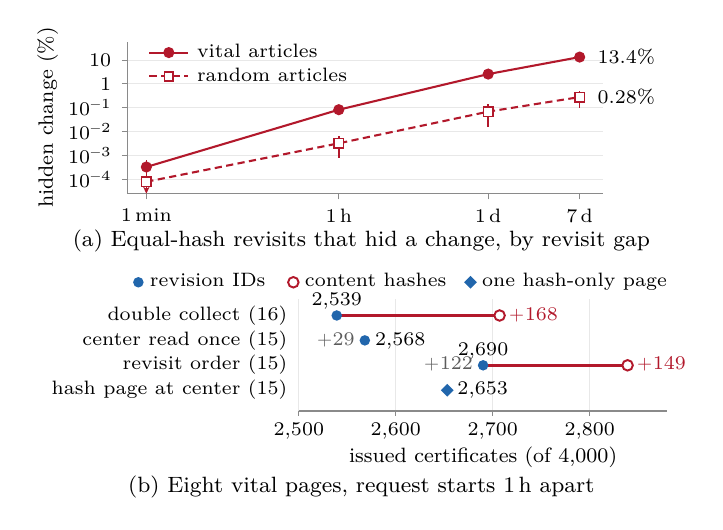
\begin{tikzpicture}[x=1pt, y=1pt]
\useasboundingbox (0,-171.20) rectangle (241.15,0);
\begin{axis}[name=a, at={(36pt,-60pt)}, anchor=south west, scale only axis,
  width=172pt, height=55pt, xmode=log, ymode=log,
  xmin=40, xmax=1.0e6, ymin=2.5e-05, ymax=60,
  xtick={60,3600,86400,604800}, xticklabels={1\,min,1\,h,1\,d,7\,d},
  ytick={1e-4,1e-3,1e-2,1e-1,1,10}, yticklabels={$10^{-4}$,$10^{-3}$,$10^{-2}$,$10^{-1}$,$1$,$10$},
  minor tick style={draw=none}, tick align=outside, tick style={rule, line width=0.4pt}, major tick length=2pt,
  axis line style={rule, line width=0.4pt}, axis lines*=left,
  ymajorgrids, grid style={black!9, line width=0.4pt},
  tick label style={font=\figsmall}, label style={font=\figlabel},
  ylabel={hidden change (\%)}, ylabel style={yshift=-3pt},
  clip=false]
\draw[fails, line width=0.55pt] (axis cs:60,8.251e-05) -- (axis cs:60,0.000660117);
\draw[fails, line width=0.55pt] (axis cs:3600,0.0669722) -- (axis cs:3600,0.100428);
\draw[fails, line width=0.55pt] (axis cs:86400,2.14164) -- (axis cs:86400,3.0942);
\draw[fails, line width=0.55pt] (axis cs:604800,11.0391) -- (axis cs:604800,15.7951);
\addplot[fails, line width=0.75pt, solid, mark=*, mark size=1.7pt, mark options={solid, fill=fails, draw=fails, line width=0.6pt}] coordinates {(60,0.000330053) (3600,0.0831055) (86400,2.58812) (604800,13.3539)};
\node[font=\figsmall, anchor=west, inner sep=0pt] at (axis cs:876960.0,13.3539) {13.4\%};
\draw[fails, line width=0.55pt, -{Stealth[length=2.6pt, width=2.4pt]}] (axis cs:60,0.000240016) -- (axis cs:60,2.5e-05);
\draw[fails, line width=0.55pt] (axis cs:3600,0.000788059) -- (axis cs:3600,0.00674001);
\draw[fails, line width=0.55pt] (axis cs:86400,0.0163413) -- (axis cs:86400,0.150279);
\draw[fails, line width=0.55pt] (axis cs:604800,0.100429) -- (axis cs:604800,0.516185);
\addplot[fails, line width=0.75pt, dash pattern=on 2.6pt off 1.6pt, mark=square*, mark size=1.7pt, mark options={solid, fill=white, draw=fails, line width=0.6pt}] coordinates {(60,7.91509e-05) (3600,0.00324853) (86400,0.0689096) (604800,0.28139)};
\node[font=\figsmall, anchor=west, inner sep=0pt] at (axis cs:876960.0,0.28139) {0.28\%};
\end{axis}
\draw[fails, line width=0.75pt, solid] (44,-9.00) -- (58,-9.00);
\filldraw[fill=fails, draw=fails, line width=0.6pt] (51,-9.00) circle (1.7pt);
\node[font=\figsmall, anchor=west, inner sep=0pt] at (61,-9.00) {\strut vital articles};
\draw[fails, line width=0.75pt, dash pattern=on 2.6pt off 1.6pt] (44,-17.60) -- (58,-17.60);
\filldraw[fill=white, draw=fails, line width=0.6pt] (51,-17.60) +(-1.6pt,-1.6pt) rectangle +(1.6pt,1.6pt);
\node[font=\figsmall, anchor=west, inner sep=0pt] at (61,-17.60) {\strut random articles};
\node[font=\figtitle, anchor=base, inner sep=0pt] at (120.57,-79.00) {(a) Equal-hash revisits that hid a change, by revisit gap};
\draw[black!9, line width=0.4pt] (98.00,-138.50) -- (98.00,-98.00);
\draw[black!9, line width=0.4pt] (133.04,-138.50) -- (133.04,-98.00);
\draw[black!9, line width=0.4pt] (168.08,-138.50) -- (168.08,-98.00);
\draw[black!9, line width=0.4pt] (203.12,-138.50) -- (203.12,-98.00);
\draw[rule, line width=0.4pt] (98.00,-138.50) -- (231.15,-138.50);
\draw[rule, line width=0.4pt] (98.00,-138.50) -- (98.00,-140.50);
\node[font=\figsmall, anchor=base, inner sep=0pt] at (98.00,-147.50) {2,500};
\draw[rule, line width=0.4pt] (133.04,-138.50) -- (133.04,-140.50);
\node[font=\figsmall, anchor=base, inner sep=0pt] at (133.04,-147.50) {2,600};
\draw[rule, line width=0.4pt] (168.08,-138.50) -- (168.08,-140.50);
\node[font=\figsmall, anchor=base, inner sep=0pt] at (168.08,-147.50) {2,700};
\draw[rule, line width=0.4pt] (203.12,-138.50) -- (203.12,-140.50);
\node[font=\figsmall, anchor=base, inner sep=0pt] at (203.12,-147.50) {2,800};
\node[font=\figlabel, anchor=base, inner sep=0pt] at (164.57,-157.00) {issued certificates (of 4,000)};
\node[font=\figsmall, anchor=east, inner sep=0pt] at (94.00,-104.00) {\strut double collect (16)};
\draw[fails, line width=1.0pt] (111.67,-104.00) -- (170.53,-104.00);
\filldraw[fill=white, draw=fails, line width=0.7pt] (170.53,-104.00) circle (1.9pt);
\node[font=\figsmall, text=fails, anchor=west, inner sep=0pt] at (174.03,-104.00) {\strut $+$168};
\fill[sound] (111.67,-104.00) circle (1.9pt);
\node[font=\figsmall, anchor=base, inner sep=0pt] at (111.67,-100.40) {2,539};
\node[font=\figsmall, anchor=east, inner sep=0pt] at (94.00,-113.00) {\strut center read once (15)};
\fill[sound] (121.83,-113.00) circle (1.9pt);
\node[font=\figsmall, anchor=west, inner sep=0pt] at (125.33,-113.00) {\strut 2,568};
\node[font=\figsmall, text=muted, anchor=east, inner sep=0pt] at (118.33,-113.00) {\strut $+$29};
\node[font=\figsmall, anchor=east, inner sep=0pt] at (94.00,-122.00) {\strut revisit order (15)};
\draw[fails, line width=1.0pt] (164.57,-122.00) -- (216.78,-122.00);
\filldraw[fill=white, draw=fails, line width=0.7pt] (216.78,-122.00) circle (1.9pt);
\node[font=\figsmall, text=fails, anchor=west, inner sep=0pt] at (220.28,-122.00) {\strut $+$149};
\fill[sound] (164.57,-122.00) circle (1.9pt);
\node[font=\figsmall, anchor=base, inner sep=0pt] at (164.57,-118.40) {2,690};
\node[font=\figsmall, text=muted, anchor=east, inner sep=0pt] at (161.07,-122.00) {\strut $+$122};
\node[font=\figsmall, anchor=east, inner sep=0pt] at (94.00,-131.00) {\strut hash page at center (15)};
\fill[sound] (151.61,-128.70) -- (153.91,-131.00) -- (151.61,-133.30) -- (149.31,-131.00) -- cycle;
\node[font=\figsmall, anchor=west, inner sep=0pt] at (155.11,-131.00) {\strut 2,653};
\fill[sound] (40.00,-92.00) circle (1.9pt);
\node[font=\figsmall, anchor=west, inner sep=0pt] at (44.00,-92.00) {\strut revision IDs};
\filldraw[fill=white, draw=fails, line width=0.7pt] (96.00,-92.00) circle (1.9pt);
\node[font=\figsmall, anchor=west, inner sep=0pt] at (100.00,-92.00) {\strut content hashes};
\fill[sound] (160.00,-89.70) -- (162.30,-92.00) -- (160.00,-94.30) -- (157.70,-92.00) -- cycle;
\node[font=\figsmall, anchor=west, inner sep=0pt] at (164.00,-92.00) {\strut one hash-only page};
\node[font=\figtitle, anchor=base, inner sep=0pt] at (120.57,-168.00) {(b) Eight vital pages, request starts 1\,h apart};
\end{tikzpicture}
\end{document}
